\documentclass[10pt]{article}
\usepackage[utf8]{inputenc}
\usepackage{fixltx2e}
\usepackage{graphicx}
\usepackage{longtable}
\usepackage{booktabs}
\usepackage{amssymb}
\usepackage{hyperref}
\usepackage{mathpazo}
\usepackage{fullpage}
\usepackage{setspace}
\usepackage{amsmath, amssymb, amscd}
\usepackage{algorithm}
\usepackage{algorithmicx}
\usepackage{algpseudocode}
\title{Spam}
\author{Jon-Michael Deldin}
\date{\today}
\begin{document}

\doublespace
\section{Introduction}
Spam is a significant problem in online communities. Spammers advertise their
products, services, viruses, and more to members of these social networks.
Social networks are targeted because they are generally free, and the spammers
can advertise to users via direct messaging or indirect communication (e.g.,
comments on a post). This severely degrades the legitimate user's experience,
affects the website's search engine ranking, and tarnishes the website's
public image.

One social network suffering from spam is
AskNature\footnote{\url{http://www.asknature.org} }. AskNature is a free,
online database of biomimetic\cite{benyus} solutions. Members can create a
profile, comment on articles, create and read articles, and participate in
forums. Unfortunately, spammers take advantage of the open user registration
and inundate the site with illegitimate accounts, such as the one shown in
Fig.~\ref{fig:spam-profile}. Since the site opened in November 2008, the staff
detected nearly 20,000 spam profiles, in contrast to almost 9,000 legitimate
profiles\footnote{As of November 28, 2012 }. The site has coped with a few
heuristics tools that check for links and HTML, but they are run only to
detect profiles -- a human still inspects and bans users.

\begin{figure}[b]
\centering
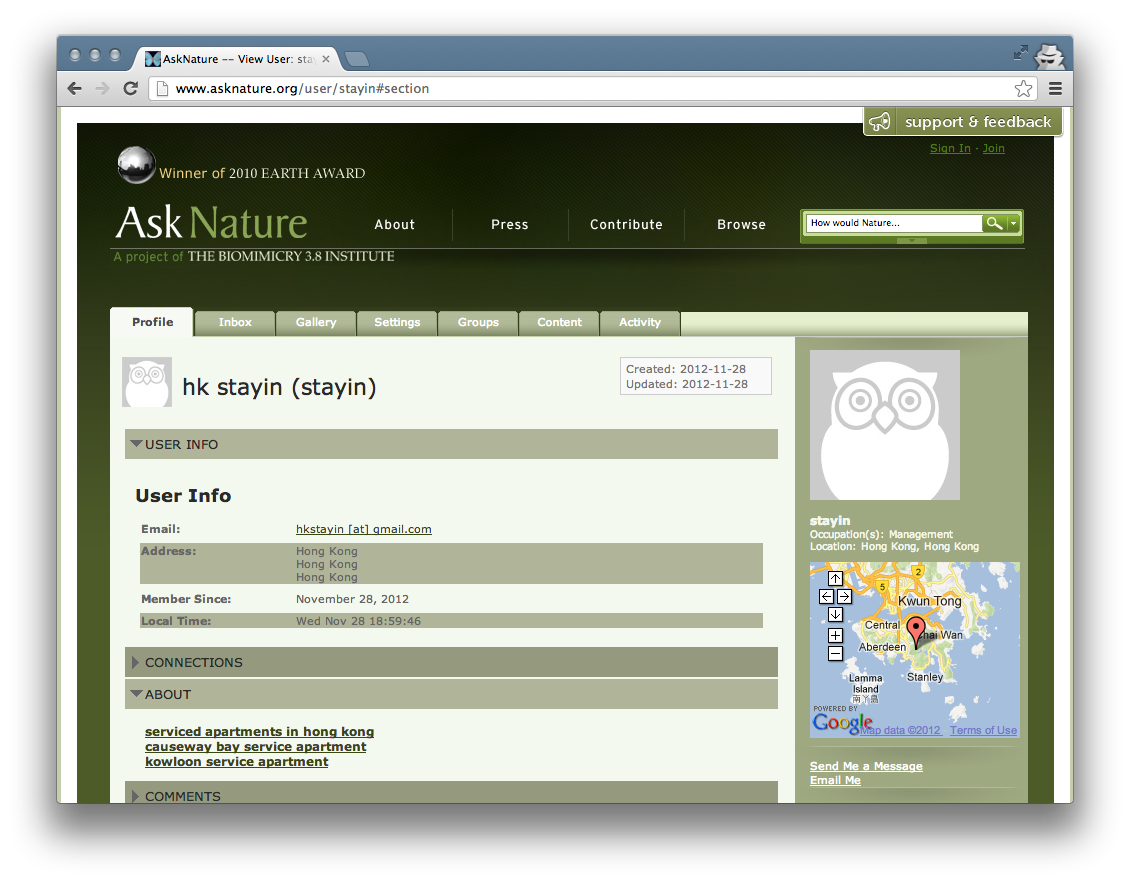
\includegraphics[width=\textwidth]{fig/spam-profile.png}
\caption{This screenshot of a spam profile shows the "about" text the spammer
enters, along with the first name ("hk"), last name ("stayin"), username
("staying"), and the spammer's address.}
\label{fig:spam-profile}
\end{figure}

% FIXME: Check again
In this project, I developed a naive Bayes classifier for detecting spam
profiles based on the user's biography\footnote{I will be using ``biography''
  and ``profile'' interchangeably.}. The goal is to determine whether
an account is spam or ham (i.e., a legitimate account) based on the plain text
of the profile. I hypothesized a unigram bag of words model where each word is
represented phonetically is more accurate than representing the words as
themselves. Matching words based on their pronunciation should capture some
misspellings, narrowing the search space of the classifier.

  To test this, I performed the following experiments:

\begin{enumerate}
  \item Determine the ratio of spam to ham yielding the highest accuracy
  \item Determine the minimum number of characters for a biography yielding
    the highest accuracy
  \item Determine which n-gram model yields better results for both word and
    character grams
\end{enumerate}

\section{Naive Bayes Classifier}
The research presented here utilizes a naive Bayes classifier to classify spam
and ham. These classifiers are very effective for classifying
documents\cite[p182]{mitchell}, especially at spam
classification\cite{which-nb}. In a naive Bayes classifier, each feature is
assumed to be independent. In this paper, I used a bag-of-words model to
capture the frequency of each word appearing in a document. In a later
section, single-word (unigram) models are evaluated against bigrams, trigrams,
and character-grams.

Additionally, these can be FIXME laplace smoothed.

\section{Evaluation}
$k$-fold cross-validation is used to compare the performance of the classifier
with different models. The algorithm is described in
Algorithm~\ref{algo:crossvalidation}. Cross-validation will return a confusion
matrix -- a table of false positives (ham marked as spam), false negatives
(spam marked as ham), true positives (spam), and true negatives
(ham)\footnote{For brevity, $fp$ will denote a false positive, $tn$ will
  denote a true negative, and so on.}.

For determining an optimal classifier, we may consider the following metrics \cite{eval}:

\begin{description}
\item[accuracy] $\frac{tp + tn}{tp + fp + fn + tn}$
\item[precision] $\frac{tp}{tp + fp}$
\item[recall] $\frac{tp}{tp + fn}$
\end{description}

Accuracy measures how well we correctly predict classes, precision
measures how well we correctly make positive predictions (a higher precision
means fewer false positives), and recall measures the sensitivity of the
classifier (a higher recall means fewer false negatives). In this paper, we
value models with a high accuracy and a high precision. We want to correctly
classify as much spam as possible, but we do not want to mistake legitimate
users for spammers as much as possible.


\begin{algorithm}
\caption{$k$-fold cross-validation described by \cite[p147]{mitchell}}
\begin{algorithmic}
\Function{CrossValidate}{data, $k$}
\State partitions $\gets$ divide data into $k$ disjoint subsets
\For{$i \gets 1 \to k$}
\State{$T \gets$ data $\setminus\ \mathrm{partitions}_i$}
\State{{\sc train}($T$)}
\State{{\sc classify}($\mathrm{partitions}_i$)}
\State \Return{confusion matrix}
\EndFor
\EndFunction
\end{algorithmic}\label{algo:crossvalidation}
\end{algorithm}

\section{Data}
The data consist of user biographies -- Unicode text fields -- spanning
2008-09-03--2012-11-28. These profiles\footnote{I will use the terms
  ``profile'' and ``biography'' interchangeably from this point forward.} are
from AskNature's MySQL database, and they were processed as described in
Algorithm~\ref{algo:preprocess} before being saved to disk as plain text files
for easier distribution. Empty profiles were not included.

With data in hand, the next step is determining the minimum number of words a
sample must contain for use in a classifier. As shown in
Table~\ref{table:corpus-stats}, the data set includes more spam accounts than
ham, and those spam accounts have fewer words per biography on average. The
wide standard deviation for both classes is explained by two factors: Users
are not required to fill out the biography field, and even if they choose to,
no stated minimum or maximum requirements exist. We will use the floor of the
minimum mean length, which is 32 words per biography. This prevents too much
data from being rejected.

Next, training and testing sets must be developed. The algorithm for doing
such is described in Algorithm~\ref{algo:segment}.

\begin{table}
  \centering
  \caption{Summary statistics for the non-empty biographies processed
    according to Algorithm~\ref{algo:preprocess}.}
  \label{table:corpus-stats}
  \begin{tabular}{lccc}
    \toprule
    Class & $N$ & Mean Length (words) & $\sigma$\\ \midrule
    Spam  & 18,588 & 32.6 & 92.4 \\
    Ham   & 3,287  & 63.7 & 104.6 \\
    \bottomrule
  \end{tabular}
\end{table}


The total corpus consists of 3,144 ham profiles and 18,461 spam profiles saved
as HTML fragments. However, for experimentation, 3,000 samples from each class
were randomly selected without replacement kept for efficiency. Each spam profile was identified by members of the
AskNature staff, and the other profiles are assumed to be ham. Each sample is
pre-processed in the following manner:
DUE TO THE DISPROPORTIONATE AMOUNT OF SPAM, IT HAS BEEN CAPPED AT 3000 by
randomly shuffling. SAME FOR HAM. and then droppingc

\begin{algorithm}
\begin{enumerate}
  \item Sanitize all HTML by retaining just the \texttt{innerHTML} (the
    content between start and closing tags). For example, \texttt{<a
      href="http://example.com">link</a>} becomes \texttt{link}.
  \item Remove all URLs
  \item Replace excess whitespace with single spaces
\end{enumerate}
\caption{Preprocessing routine for biographies}
\label{algo:preprocess}
\end{algorithm}

Samples with fewer than five characters after cleaning were rejected, as there
is little to be gained from matching an abbreviation or a single short word.

\section{Methods}

In this section, I describe the methods used to determine an optimal naive
Bayes classifier for classifying spam user profiles on AskNature.

\subsection{Determining the ratio of spam to ham}
An important first step is determining what ratio of spam
To evaluate what ratio of spam to ham would yield a stronger classifier, the
following test was performed.

\begin{algorithm}
  \caption{Determine the ratio of spam:ham messages with the greatest accuracy.}
  \begin{algorithmic}
  \Function{FindBestRatio}{samples, $n$}
  \Comment{Takes a set of $n$ samples}
  \State spam $\gets$ {\sc shuffle}(samples $\setminus $ ham)
  \Comment{Randomizes the order of samples}
  \State ham $\gets$ {\sc shuffle}(samples $\setminus $ spam)
  \State best-accuracy $\gets 0$
  \State best-ratio $\gets \emptyset$
  \\

  \For{$i \gets 0.0 \to 1.0$, step $\gets 0.01$}
  \State ham-ratio $\gets ni$
  \State spam-ratio $\gets n(1 - i)$
  \State limited-samples $\gets$ {\sc take}(ham, ham-ratio) $\cup$ {\sc take}(spam, spam-ratio)
  \\

  \State {\sc cross-validate}(limited-samples)

  \If{accuracy > best-accuracy}
  \State{best-accuracy $\gets$ accuracy}
  \State{best-ratio $\gets$ \{ham-ratio, spam-ratio\}}
  \EndIf
  \EndFor
  \State \Return{best-ratio, best-accuracy}
    \EndFunction
  \end{algorithmic}\label{algo}
\end{algorithm}
\subsubsection{Table of results}
\label{sec-2-2-1}

5 iterations of 3000 cap. Mean and standard devs.
\begin{tabular}{lllllllllllllll}
step & meanAcc & sdAcc & meanPrec & sdPrec & meanRecall & sdRecall & meanTp & sdTp & meanTn & sdTn & meanFp & sdFp & meanFn & sdFn \\
0.810 & 0.886 & 0.005 & 0.894 & 0.004 & 0.975 & 0.002 & 2370.000 & 5.568 & 289.333 & 9.815 & 280.667 & 9.815 & 60.000 & 5.568 \\
0.820 & 0.881 & 0.004 & 0.894 & 0.003 & 0.969 & 0.001 & 2384.667 & 3.215 & 257.333 & 9.815 & 282.667 & 9.815 & 75.333 & 3.215 \\
0.830 & 0.877 & 0.005 & 0.895 & 0.004 & 0.964 & 0.002 & 2400.333 & 5.859 & 229.333 & 10.017 & 280.667 & 10.017 & 89.667 & 5.859 \\
0.840 & 0.871 & 0.004 & 0.896 & 0.003 & 0.958 & 0.001 & 2414.333 & 2.887 & 198.667 & 8.083 & 281.333 & 8.083 & 105.667 & 2.887 \\
0.850 & 0.867 & 0.003 & 0.897 & 0.002 & 0.953 & 0.002 & 2431.333 & 4.933 & 169.667 & 4.933 & 280.333 & 4.933 & 118.667 & 4.933 \\
0.860 & 0.862 & 0.004 & 0.898 & 0.001 & 0.948 & 0.004 & 2446.333 & 11.150 & 140.667 & 2.517 & 279.333 & 2.517 & 133.667 & 11.150 \\
0.870 & 0.855 & 0.005 & 0.897 & 0.001 & 0.943 & 0.004 & 2460.000 & 10.817 & 106.333 & 3.215 & 283.667 & 3.215 & 150.000 & 10.817 \\
0.880 & 0.850 & 0.005 & 0.896 & 0.001 & 0.938 & 0.006 & 2477.333 & 15.373 & 73.333 & 0.577 & 286.667 & 0.577 & 162.667 & 15.373
\end{tabular}
\subsubsection{Selection}
\label{sec-2-2-2}
\subsubsection{Preprocessing}
\label{sec-2-2-3}
\subsubsection{Determining the Minimum Number of Characters}
\label{sec-2-2-4}

We needed to prune. We ran a Naive Bayes Classifier with both unigram and
bigram word models to determine that 18 character sized bodies would give the
greatest accuracy (94.86\% accuracy on 1,000 sample, k=100 cross validation)
\subsection{Naïve Bayes Classifier}
\label{sec-2-3}
\subsubsection{Bag of Words}
\label{sec-2-3-1}
\subsubsection{Bag of Phonetics}
\label{sec-2-3-2}
\subsection{Implementation}
\label{sec-2-4}
\section{Results}
\label{sec-3}
\subsection{F-score}
\label{sec-3-1}

STASTICAL SIGNIFICANCE OF ACCURACY DIFFERENCE
\section{Discussion}
\label{sec-4}
\section{Conclusion}
\label{sec-5}



\bibliographystyle{plain}
\bibliography{refs}

\end{document}
